\documentclass[fleqn,reqno,10pt,draft]{article}



%========================================
% Packages
%========================================

\usepackage[]{helpers/mypackages}

\bibliography{MyRefGlobal}

%\usepackage[garamond]{mathdesign}




%========================================
% Theorem Environments
%========================================

\usepackage{helpers/myenvironments}


%========================================
% Commands
%========================================

\usepackage{helpers/mycommands}


%========================================
% Page Layout
%========================================
% \renewcommand{\baselinestretch}{1.1} % multiplies vertical distance between lines in a paragraph
% \setlength{\parskip}{1ex plus 0.4ex minus 0.1ex}
% \addtolength{\voffset}{-1.7cm} \addtolength{\hoffset}{-1.5cm}
% \addtolength{\textwidth}{3.1cm} \addtolength{\textheight}{2.3cm}
% \addtolength{\voffset}{-1cm} \addtolength{\hoffset}{-0.5cm}
% \addtolength{\textwidth}{1cm} \addtolength{\textheight}{2cm}
% \setlength{\parindent}{0cm} % set paragraph indentation

%========================================
% More Layout
%========================================

% Itemize
\renewcommand{\labelitemi}{\large{$\mathbf{\cdot}$}}    % itemize symbols
\renewcommand{\labelitemii}{\large{$\mathbf{\cdot}$}}
\renewcommand{\labelitemiii}{\large{$\mathbf{\cdot}$}}
\renewcommand{\labelitemiv}{\large{$\mathbf{\cdot}$}}

% Description
\renewcommand{\descriptionlabel}[1]{\hspace\labelsep\textsc{#1}}

% Figure Captions
\usepackage{caption} % use corresponding myfiguresize!
\setlength{\captionmargin}{20pt}
\renewcommand{\captionfont}{\small}
\setlength{\belowcaptionskip}{7pt} % standard is 0pt

% Equationnumbering
%\numberwithin{equation}{section}

% sectioning
% \usepackage{sectsty}
% \chapterfont{\rmfamily\mdseries\Large\raggedleft}
% \sectionfont{\rmfamily\mdseries\large\nohang}
% \subsectionfont{\rmfamily\mdseries\normalsize\nohang}
% \subsubsectionfont{\rmfamily\mdseries\normalsize\itshape\nohang}
% \paragraphfont{\rmfamily\mdseries\normalsize\textsc}

% for indentation of section headings:
%\sectionfont{\hspace*{-2.3em}\rmfamily\mdseries\bfseries\large\nohang\raggedright}

%========================================
% Special for this Document
%========================================

\newcommand{\lit}{\ensuremath{\text{\textsc{lit}}}}
\newcommand{\glb}{\ensuremath{\text{\textsc{glb}}}}
\newcommand{\loc}{\ensuremath{\text{\textsc{loc}}}}

%========================================
% Document
%========================================


\title{Scalar Items in Embedded Positions}

\author{Michael Franke}
\date{\today}

\begin{document}

\maketitle

\section{Motivation}

\begin{itemize}
\item we are interested in studying potential global/local
  implicatures for sentences of the forms:
  \begin{exe}
    \ex 
      \begin{xlist}
        \ex All of the $X$'s are related to some of the $Y$'s.
        \ex Exactly one of the $X$'s is related to some of the $Y$'s.
        \ex Exactly one of the $Y$'s is related to all of the $Y$'s.
      \end{xlist}
  \end{exe}
\end{itemize}

\subsection{Global Implicatures}
\label{sec:global-implicatures}

\begin{itemize}
\item a \textsc{global implicature} of a sentence is derived by
  replacing one scalar item with its scale mates and negating the
  resulting sentence:
  \begin{exe}
    \ex \label{bsp:All_Some-Global} All of the $X$'s are related to some of the $Y$'s.
      \begin{xlist}
      \ex All of the $X$'s are related to some of the $Y$'s and
        \dots 
       \ex \dots it's
        not the case that all of the $X$'s are related to all of the $Y$'s.
      \end{xlist}
    \ex \label{bsp:Exactly_1_Some-Global} Exactly one of the $X$'s is related to some of the $Y$'s.
      \begin{xlist}
        \ex Exactly one of the $X$'s is related to some of the $Y$'s
          and \dots 
        \ex  \dots it's not the case that exactly one of the $X$'s is
          related to all of the $Y$'s.
      \end{xlist}
    \ex \label{bsp:Exactly_1_All-Global} Exactly one of the $Y$'s is related to all of the $Y$'s.
      \begin{xlist}
        \ex Exactly one of the $X$'s is related to all of the $Y$'s
          and \dots 
        \ex  \dots it's not the case that exactly one of the $X$'s is
          related to some of the $Y$'s.
      \end{xlist}
  \end{exe}
\item the global implicatures in (\ref{bsp:All_Some-Global}) and
  (\ref{bsp:Exactly_1_Some-Global}) are attested by all current formal
  theories of quantity implicature
\item we are interested in whether this prediction is borne out;
  previous experimentation supports this
\item we are also interested in whether we find support for the global
  implicature in (\ref{bsp:Exactly_1_All-Global}), which some theories
  predict
  \citep[e.g.][]{Sauerland2004:Scalar-Implicat,Fox2007:Free-Choice-and}
  and others don't \citep{HornDivisionofLabor1984};\draftnote{need to
    check in detail who predicts what} this case has not been
  investigated yet
\end{itemize}



\subsection{Local Implicatures}
\label{sec:local-implicatures}

\begin{itemize}
\item a \textsc{local implicature} of a sentence is derived by
  inserting into any appropriate scope site an exhaustifity operator
  akin to the workings of \emph{only},\draftnote{there is some due
    variation in formulation of this kind of approach}
\item all global implicatures are local implicatures, but additionally
  for our target sentences we may derive:
  \begin{exe}
    \ex \label{bsp:All-some-local} All of the $X$'s are related to some of the $Y$'s.
      \begin{xlist}
      \ex All of the $X$'s are related to some but not all of the $Y$'s.
      \end{xlist}
    \ex \label{bsp:Exactly-1-some-local} Exactly 1 of the $X$'s is related to some of the $Y$'s.
      \begin{xlist}
      \ex Exactly 1 of the $X$'s is related to some but not all of the $Y$'s.
      \end{xlist}
  \end{exe}
\item we are interested in whether these local implicatures are
  attested; previous studies have presented diverging evidence for
  this: \citet{GeurtsPouscoulous2009:Embedded-Implic} provide evidence
  \emph{against}; \citet{ChemlaSpector2010:Experimental-Ev} provide evidence
  \emph{for} these inferences
\end{itemize}

\section{Material}
\label{sec:material}

\begin{itemize}
\item we apply a truth-value judgement task, under the supposition
  that implicatures, when drawn, inform truth-judgements
\item we speak of a possible ``reading'' of a sentence: whether a
  global and/or local implicature is drawn
  \begin{itemize}
  \item literal reading: literally true \hfill (\lit)
  \item global reading: global implicature true \hfill (\glb)
  \item local reading: local implicature true \hfill (\loc)
  \end{itemize}
\item we present each of the three sentences with enough pictures to
  distinguish any possible reading
\item since there may be entailment relations between these
  ``readings'', the space of possibilities is rather restricted\\
  (e.g., obviously, the global reading always entails the literal reading)
\end{itemize}

\subsection{Case: ``All of the $X$'s are related to some of the $Y$'s.''}
\label{sec:case:-all-some}

\begin{itemize}
\item entailment relations in this case are: $\loc
  \Rightarrow \glb \Rightarrow \lit$
\item we can thus distinguish four cases:
  \begin{center}
    \begin{tabular}{lccc}
      \toprule
      & \textsc{lit} & \textsc{glb} & \textsc{loc} \\ \midrule
      Case 1 & 1 & 1 & 1 \\
      Case 2 & 1 & 1 & 0 \\
      Case 3 & 1 & 0 & 0 \\
      Case 4 & 0 & 0 & 0 \\ \bottomrule
    \end{tabular}
  \end{center}
\end{itemize}

\subsubsection{Pictures}
\label{sec:pictures}

\begin{itemize}

\item these cases can be tested for with the following
  diagrams:
  \begin{itemize}
  \item Case 1 (true-true-true): 
  
    \begin{center}
      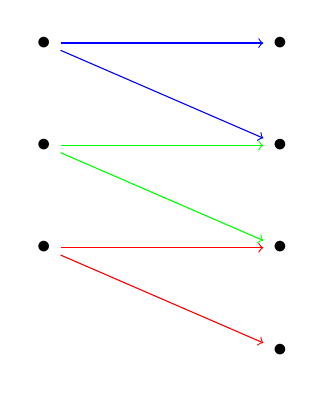
\begin{tikzpicture}[node distance = 1.3cm]
        % Nodes

        \node (X-1) {$\Large{\bullet}$};

        \node (X-2) [below of = X-1] {$\Large{\bullet}$};

        \node (X-3) [below of = X-2] {$\Large{\bullet}$};

        \node (Y-1) [right of = X-1, node distance = 3cm]{$\Large{\bullet}$};

        \node (Y-2) [below of = Y-1] {$\Large{\bullet}$};

        \node (Y-3) [below of = Y-2] {$\Large{\bullet}$};

        \node (Y-4) [below of = Y-3] {$\Large{\bullet}$};

        % Arrows

        \path [draw=blue,->] (X-1) -> (Y-1);

        \path [draw=blue,->] (X-1) -> (Y-2);


        \path [draw=green,->] (X-2) -> (Y-2);

        \path [draw=green,->] (X-2) -> (Y-3);


        \path [draw=red,->] (X-3) -> (Y-3);

        \path [draw=red,->] (X-3) -> (Y-4);

      \end{tikzpicture}
    \end{center}

  \item Case 2 (true-true-false):
    
    \begin{center}
      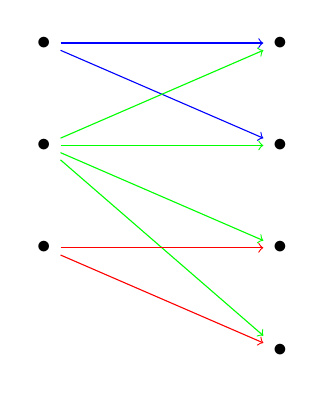
\begin{tikzpicture}[node distance = 1.3cm]
        % Nodes

        \node (X-1) {$\Large{\bullet}$};

        \node (X-2) [below of = X-1] {$\Large{\bullet}$};

        \node (X-3) [below of = X-2] {$\Large{\bullet}$};

        \node (Y-1) [right of = X-1, node distance = 3cm]{$\Large{\bullet}$};

        \node (Y-2) [below of = Y-1] {$\Large{\bullet}$};

        \node (Y-3) [below of = Y-2] {$\Large{\bullet}$};

        \node (Y-4) [below of = Y-3] {$\Large{\bullet}$};

        % Arrows

        \path [draw=blue,->] (X-1) -> (Y-1);

        \path [draw=blue,->] (X-1) -> (Y-2);


        \path [draw=green,->] (X-2) -> (Y-1);

        \path [draw=green,->] (X-2) -> (Y-2);

        \path [draw=green,->] (X-2) -> (Y-3);

        \path [draw=green,->] (X-2) -> (Y-4);


        \path [draw=red,->] (X-3) -> (Y-3);

        \path [draw=red,->] (X-3) -> (Y-4);

      \end{tikzpicture}

    \end{center}
    \item Case 3 (true-false-false):

\begin{center}
      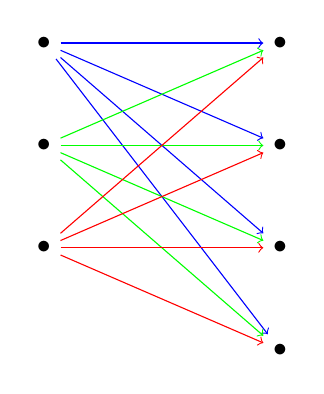
\begin{tikzpicture}[node distance = 1.3cm]
        % Nodes

        \node (X-1) {$\Large{\bullet}$};

        \node (X-2) [below of = X-1] {$\Large{\bullet}$};

        \node (X-3) [below of = X-2] {$\Large{\bullet}$};

        \node (Y-1) [right of = X-1, node distance = 3cm]{$\Large{\bullet}$};

        \node (Y-2) [below of = Y-1] {$\Large{\bullet}$};

        \node (Y-3) [below of = Y-2] {$\Large{\bullet}$};

        \node (Y-4) [below of = Y-3] {$\Large{\bullet}$};

        % Arrows

        \path [draw=blue,->] (X-1) -> (Y-1);

        \path [draw=blue,->] (X-1) -> (Y-2);

        \path [draw=blue,->] (X-1) -> (Y-3);

        \path [draw=blue,->] (X-1) -> (Y-4);


        \path [draw=green,->] (X-2) -> (Y-1);

        \path [draw=green,->] (X-2) -> (Y-2);

        \path [draw=green,->] (X-2) -> (Y-3);

        \path [draw=green,->] (X-2) -> (Y-4);



        \path [draw=red,->] (X-3) -> (Y-1);

        \path [draw=red,->] (X-3) -> (Y-2);

        \path [draw=red,->] (X-3) -> (Y-3);

        \path [draw=red,->] (X-3) -> (Y-4);


      \end{tikzpicture}

    \end{center}

    \item Case 4 (false-false-false):

\begin{center}
      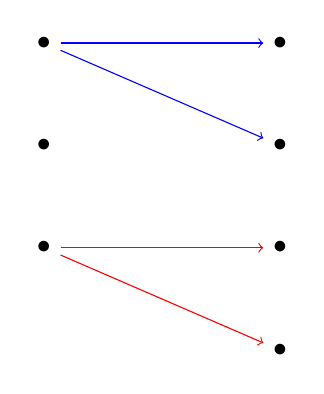
\begin{tikzpicture}[node distance = 1.3cm]
        % Nodes

        \node (X-1) {$\Large{\bullet}$};

        \node (X-2) [below of = X-1] {$\Large{\bullet}$};

        \node (X-3) [below of = X-2] {$\Large{\bullet}$};

        \node (Y-1) [right of = X-1, node distance = 3cm]{$\Large{\bullet}$};

        \node (Y-2) [below of = Y-1] {$\Large{\bullet}$};

        \node (Y-3) [below of = Y-2] {$\Large{\bullet}$};

        \node (Y-4) [below of = Y-3] {$\Large{\bullet}$};

        % Arrows

        \path [draw=blue,->] (X-1) -> (Y-1);

        \path [draw=blue,->] (X-1) -> (Y-2);


        \path [draw=red,->] (X-3) -> (Y-3);

        \path [draw=red,->] (X-3) -> (Y-4);


      \end{tikzpicture}

    \end{center}

  \end{itemize}
\end{itemize}

\subsubsection{Sentence Items}
\label{sec:sentence-items}

\begin{exe}
  \ex
    \begin{xlist}
    \ex Für jeden dieser Anwälte gilt: er vertritt einige dieser
      Angeklagten.
    \ex Für jedes dieser Kinder gilt: es mag einige dieser
      Speisen.
    \ex Für jeden dieser Kritiker gilt: er lobte einige dieser
      Aufführungen.
    \ex Für jede dieser Tennisspielerinnen gilt: sie hat schon
      einige dieser Turniere gewonnen.
    \ex Für jede dieser Künstlerinnen gilt: sie stellt in einigen
      dieser Museen aus.
    \ex Für jeden dieser Jungen gilt: er ist mit einigen dieser
      Mädchen befreundet.
    \ex Für jeden dieser Fußballfans gilt: er hat einige dieser
      Spiele gesehen.
    \ex Für jeden dieser Touristen gilt: er hat bereits einige dieser
      Länder bereist.
    \ex Für jeden dieser Bergsteiger gilt: er hat bereits einige dieser
      Gipfel erklommen.
    \ex Für jeden dieser Musikliebhaber gilt: er mag einige
      dieser Komponisten.
    \ex Für jeden dieser Schauspieler gilt: er hat bereits mit einigen dieser
      Regisseure zusammengearbeitet.
    \end{xlist}
\end{exe}

\subsection{Case: ``Exactly one of the $X$'s is related to some of the
  $Y$'s.''}
\label{sec:case:-exactly1-some}

\begin{itemize}
\item entailment relations in this case are:
  \begin{enumerate}[(i)]
  \item $\glb \Rightarrow \lit$
  \item $\glb \Rightarrow \loc$
  \item $\loc \Rightarrow \neg \lit$
  \end{enumerate}
\item so we distinguish the following four cases:
\begin{center}
    \begin{tabular}{lccc}
      \toprule
      & \textsc{lit} & \textsc{glb} & \textsc{loc} \\ \midrule
      Case 1 & 1 & 1 & 1 \\
      Case 2 & 0 & 0 & 1 \\
      Case 3 & 1 & 0 & 0 \\
      Case 4 & 0 & 0 & 0 \\ \bottomrule
    \end{tabular}
  \end{center}

\end{itemize}

\subsubsection{Pictures}
\label{sec:pictures}

\begin{itemize}

\item these cases can be tested for with the following
  diagrams:
  \begin{itemize}
  \item Case 1 (true-true-true): 
  
    \begin{center}
      \begin{tikzpicture}[node distance = 1.3cm]
        % Nodes

        \node (X-1) {$\Large{\bullet}$};

        \node (X-2) [below of = X-1] {$\Large{\bullet}$};

        \node (X-3) [below of = X-2] {$\Large{\bullet}$};

        \node (Y-1) [right of = X-1, node distance = 3cm]{$\Large{\bullet}$};

        \node (Y-2) [below of = Y-1] {$\Large{\bullet}$};

        \node (Y-3) [below of = Y-2] {$\Large{\bullet}$};

        \node (Y-4) [below of = Y-3] {$\Large{\bullet}$};

        % Arrows

        \path [draw=blue,->] (X-1) -> (Y-1);

        \path [draw=blue,->] (X-1) -> (Y-2);

      \end{tikzpicture}
    \end{center}
  \item Case 2 (false-false-true): 
  
    \begin{center}
      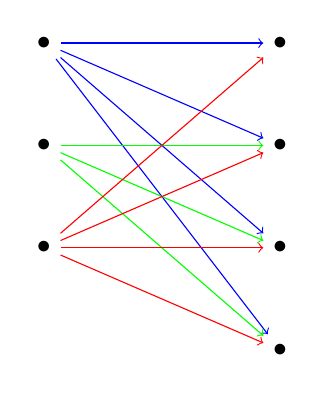
\begin{tikzpicture}[node distance = 1.3cm]
        % Nodes

        \node (X-1) {$\Large{\bullet}$};

        \node (X-2) [below of = X-1] {$\Large{\bullet}$};

        \node (X-3) [below of = X-2] {$\Large{\bullet}$};

        \node (Y-1) [right of = X-1, node distance = 3cm]{$\Large{\bullet}$};

        \node (Y-2) [below of = Y-1] {$\Large{\bullet}$};

        \node (Y-3) [below of = Y-2] {$\Large{\bullet}$};

        \node (Y-4) [below of = Y-3] {$\Large{\bullet}$};

        % Arrows

        \path [draw=blue,->] (X-1) -> (Y-1);

        \path [draw=blue,->] (X-1) -> (Y-2);

        \path [draw=blue,->] (X-1) -> (Y-3);

        \path [draw=blue,->] (X-1) -> (Y-4);



        \path [draw=green,->] (X-2) -> (Y-2);

        \path [draw=green,->] (X-2) -> (Y-3);

        \path [draw=green,->] (X-2) -> (Y-4);



        \path [draw=red,->] (X-3) -> (Y-1);

        \path [draw=red,->] (X-3) -> (Y-2);

        \path [draw=red,->] (X-3) -> (Y-3);

        \path [draw=red,->] (X-3) -> (Y-4);

      \end{tikzpicture}
    \end{center}
  \item Case 3 (true-false-false): 
  
    \begin{center}
      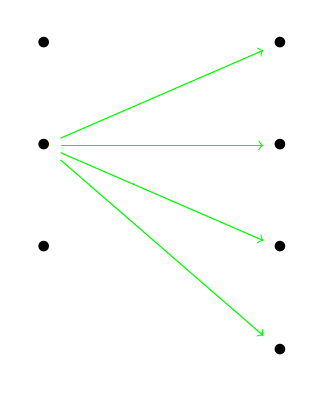
\begin{tikzpicture}[node distance = 1.3cm]
        % Nodes

        \node (X-1) {$\Large{\bullet}$};

        \node (X-2) [below of = X-1] {$\Large{\bullet}$};

        \node (X-3) [below of = X-2] {$\Large{\bullet}$};

        \node (Y-1) [right of = X-1, node distance = 3cm]{$\Large{\bullet}$};

        \node (Y-2) [below of = Y-1] {$\Large{\bullet}$};

        \node (Y-3) [below of = Y-2] {$\Large{\bullet}$};

        \node (Y-4) [below of = Y-3] {$\Large{\bullet}$};

        % Arrows

        \path [draw=green,->] (X-2) -> (Y-1);

        \path [draw=green,->] (X-2) -> (Y-2);

        \path [draw=green,->] (X-2) -> (Y-3);

        \path [draw=green,->] (X-2) -> (Y-4);

      \end{tikzpicture}
    \end{center}
  \item Case 3 (false-false-false): 
  
    \begin{center}
      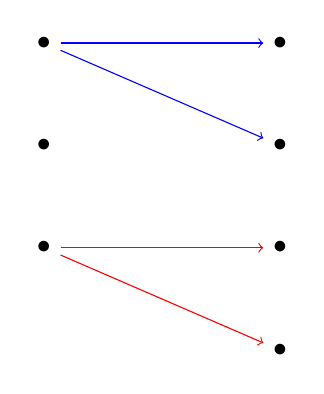
\begin{tikzpicture}[node distance = 1.3cm]
        % Nodes

        \node (X-1) {$\Large{\bullet}$};

        \node (X-2) [below of = X-1] {$\Large{\bullet}$};

        \node (X-3) [below of = X-2] {$\Large{\bullet}$};

        \node (Y-1) [right of = X-1, node distance = 3cm]{$\Large{\bullet}$};

        \node (Y-2) [below of = Y-1] {$\Large{\bullet}$};

        \node (Y-3) [below of = Y-2] {$\Large{\bullet}$};

        \node (Y-4) [below of = Y-3] {$\Large{\bullet}$};

        % Arrows

        \path [draw=blue,->] (X-1) -> (Y-1);

        \path [draw=blue,->] (X-1) -> (Y-2);


        \path [draw=red,->] (X-3) -> (Y-3);

        \path [draw=red,->] (X-3) -> (Y-4);

      \end{tikzpicture}
    \end{center}

  \end{itemize}
\end{itemize}

\subsubsection{Sentence Items}
\label{sec:sentence-items}

\begin{exe}
  \ex
    \begin{xlist}
    \ex Für genau einen dieser Anwälte gilt: er vertritt einige dieser
      Angeklagten.
    \ex Für genau eines dieser Kinder gilt: es mag einige dieser
      Speisen.
    \ex Für genau einen dieser Kritiker gilt: er lobte einige dieser
      Aufführungen.
    \ex Für genau eine dieser Tennisspielerinnen gilt: sie hat schon
      einige dieser Turniere gewonnen.
    \ex Für genau eine dieser Künstlerinnen gilt: sie stellt in einigen
      dieser Museen aus.
    \ex Für genau einen dieser Jungen gilt: er ist mit einigen dieser
      Mädchen befreundet.
    \ex Für genau einen dieser Fußballfans gilt: er hat einige dieser
      Spiele gesehen.
    \ex Für genau einen dieser Touristen gilt: er hat bereits einige dieser
      Länder bereist.
    \ex Für genau einen dieser Bergsteiger gilt: er hat bereits einige dieser
      Gipfel erklommen.
    \ex Für genau einen dieser Musikliebhaber gilt: er mag einige
      dieser Komponisten.
    \ex Für genau einen dieser Schauspieler gilt: er hat bereits mit einigen dieser
      Regisseure zusammengearbeitet.
    \end{xlist}
\end{exe}


\subsection{Case: ``Exactly one of the $X$'s is related to all of the
  $Y$'s.''}
\label{sec:case:-exactly1-all}

\begin{itemize}
\item entailment relations in this case are trivial: $\glb \Rightarrow \lit$
\item so we distinguish the following three cases:
\begin{center}
    \begin{tabular}{lcc}
      \toprule
      & \textsc{lit} & \textsc{glb} \\ \midrule
      Case 1 & 1 & 1  \\
      Case 2 & 1 & 0  \\
      Case 3 & 0 & 0  \\ \bottomrule
    \end{tabular}
  \end{center}
\end{itemize}

\subsubsection{Pictures}
\label{sec:pictures}

\begin{itemize}
\item these cases can be tested for with the following
  diagrams:
  \begin{itemize}
  \item Case 1 (true-true): 
  
    \begin{center}
      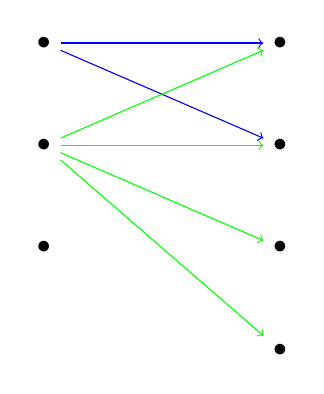
\begin{tikzpicture}[node distance = 1.3cm]
        % Nodes

        \node (X-1) {$\Large{\bullet}$};

        \node (X-2) [below of = X-1] {$\Large{\bullet}$};

        \node (X-3) [below of = X-2] {$\Large{\bullet}$};

        \node (Y-1) [right of = X-1, node distance = 3cm]{$\Large{\bullet}$};

        \node (Y-2) [below of = Y-1] {$\Large{\bullet}$};

        \node (Y-3) [below of = Y-2] {$\Large{\bullet}$};

        \node (Y-4) [below of = Y-3] {$\Large{\bullet}$};

        % Arrows

        \path [draw=blue,->] (X-1) -> (Y-1);

        \path [draw=blue,->] (X-1) -> (Y-2);


        \path [draw=green,->] (X-2) -> (Y-1);

        \path [draw=green,->] (X-2) -> (Y-2);

        \path [draw=green,->] (X-2) -> (Y-3);

        \path [draw=green,->] (X-2) -> (Y-4);

      \end{tikzpicture}
    \end{center}
  \item Case 2 (true-false): 
  
    \begin{center}
      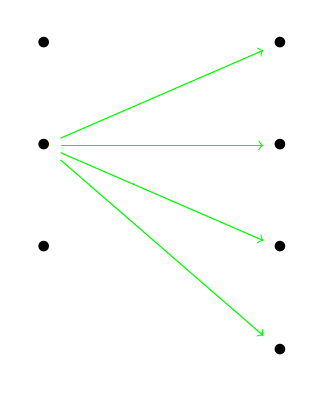
\begin{tikzpicture}[node distance = 1.3cm]
        % Nodes

        \node (X-1) {$\Large{\bullet}$};

        \node (X-2) [below of = X-1] {$\Large{\bullet}$};

        \node (X-3) [below of = X-2] {$\Large{\bullet}$};

        \node (Y-1) [right of = X-1, node distance = 3cm]{$\Large{\bullet}$};

        \node (Y-2) [below of = Y-1] {$\Large{\bullet}$};

        \node (Y-3) [below of = Y-2] {$\Large{\bullet}$};

        \node (Y-4) [below of = Y-3] {$\Large{\bullet}$};

        % Arrows

        \path [draw=green,->] (X-2) -> (Y-1);

        \path [draw=green,->] (X-2) -> (Y-2);

        \path [draw=green,->] (X-2) -> (Y-3);

        \path [draw=green,->] (X-2) -> (Y-4);


      \end{tikzpicture}
    \end{center}
  \item Case 3 (false-false): 
  
    \begin{center}
      \begin{tikzpicture}[node distance = 1.3cm]
        % Nodes

        \node (X-1) {$\Large{\bullet}$};

        \node (X-2) [below of = X-1] {$\Large{\bullet}$};

        \node (X-3) [below of = X-2] {$\Large{\bullet}$};

        \node (Y-1) [right of = X-1, node distance = 3cm]{$\Large{\bullet}$};

        \node (Y-2) [below of = Y-1] {$\Large{\bullet}$};

        \node (Y-3) [below of = Y-2] {$\Large{\bullet}$};

        \node (Y-4) [below of = Y-3] {$\Large{\bullet}$};

        % Arrows

        \path [draw=blue,->] (X-1) -> (Y-1);

        \path [draw=blue,->] (X-1) -> (Y-2);

      \end{tikzpicture}
    \end{center}
  \item Case 4 (false-false):\draftnote{we wanted to use two false
      conditions here, to fill the data set with four pictures for
      each sentence}
  
    \begin{center}
      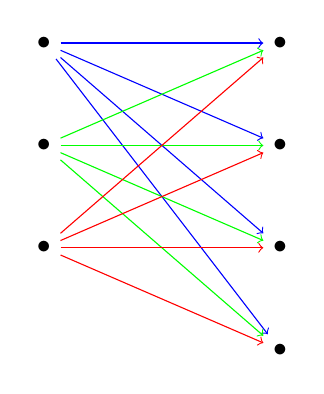
\begin{tikzpicture}[node distance = 1.3cm]
        % Nodes

        \node (X-1) {$\Large{\bullet}$};

        \node (X-2) [below of = X-1] {$\Large{\bullet}$};

        \node (X-3) [below of = X-2] {$\Large{\bullet}$};

        \node (Y-1) [right of = X-1, node distance = 3cm]{$\Large{\bullet}$};

        \node (Y-2) [below of = Y-1] {$\Large{\bullet}$};

        \node (Y-3) [below of = Y-2] {$\Large{\bullet}$};

        \node (Y-4) [below of = Y-3] {$\Large{\bullet}$};

        % Arrows

        \path [draw=blue,->] (X-1) -> (Y-1);

        \path [draw=blue,->] (X-1) -> (Y-2);

        \path [draw=blue,->] (X-1) -> (Y-3);

        \path [draw=blue,->] (X-1) -> (Y-4);


        \path [draw=green,->] (X-2) -> (Y-1);

        \path [draw=green,->] (X-2) -> (Y-2);

        \path [draw=green,->] (X-2) -> (Y-3);

        \path [draw=green,->] (X-2) -> (Y-4);



        \path [draw=red,->] (X-3) -> (Y-1);

        \path [draw=red,->] (X-3) -> (Y-2);

        \path [draw=red,->] (X-3) -> (Y-3);

        \path [draw=red,->] (X-3) -> (Y-4);

      \end{tikzpicture}
    \end{center}

  \end{itemize}
\end{itemize}

\subsubsection{Sentence Items}
\label{sec:sentence-items}

\begin{exe}
  \ex
    \begin{xlist}
    \ex Für genau einen dieser Anwälte gilt: er vertritt jeden
      dieser Angeklagten.
    \ex Für genau eines dieser Kinder gilt: es mag jede dieser
      Speisen.
    \ex Für genau einen dieser Kritiker gilt: er lobte jede dieser
      Aufführungen.
    \ex Für genau eine dieser Tennisspielerinnen gilt: sie hat schon
      jedes dieser Turniere gewonnen.
    \ex Für genau eine dieser Künstlerinnen gilt: sie stellt in jedem
      dieser Museen aus.
    \ex Für genau einen dieser Jungen gilt: er ist mit jedem dieser
      Mädchen befreundet.
    \ex Für genau einen dieser Fußballfans gilt: er hat jedes dieser
      Spiele gesehen.
    \ex Für genau einen dieser Touristen gilt: er hat bereits jedes dieser
      Länder bereist.
    \ex Für genau einen dieser Bergsteiger gilt: er hat bereits jeden dieser
      Gipfel erklommen.
    \ex Für genau einen dieser Musikliebhaber gilt: er mag jeden
      dieser Komponisten.
    \ex Für genau einen dieser Schauspieler gilt: er hat bereits mit jeden dieser
      Regisseure zusammengearbeitet.
    \end{xlist}
\end{exe}

\newpage

\section{Thoughts on Cumulative Readings}
\label{sec:thoughts-cumul-read}

\begin{itemize}
\item there may be a problem in our design from cumulative readings of (\ref{bsp:All_Some-Global})
\item under a cumulative reading, a sentence like
  (\ref{bsp:All_Some-Global}) means that the group of $X$'s \emph{as a
  whole} is connected to some of the $Y$'s
\item there are three relevant possible (disjoint) state distinctions
  for this reading:
  \begin{itemize}
  \item false-condition: group of $X$'s is connected to none of the $Y$'s; no
    arrows whatsoever
  \item literally-true-condition: group of $X$' is connected to all of
    the $Y$'s
  \item implicature-condition: group of $X$' is connected to
    some-but-not-all of the 
    $Y$'s
  \end{itemize}
\item the potential problem is that subjects' \emph{true}/\emph{false}
  judgements could be based on these cumulative readings (with/without
  implicature) and thus obscure whether they apply local or global readings
\item in particular, subjects who answer \emph{false} in cases 2 and 3
  might do so based on the cumulative reading with implicature, so
  that we might not know whether these judgements reflect on the
  potential implicatures of the non-cumulative readings
\item there is no way we can present a picture that could illicit
  judgements that would let us differentiate between cumulative and
  non-cumulative readings in cases 2 and 3
\item \emph{but} we can assess whether cumulative readings are
  available in two ways:
  \begin{itemize}
  \item under a cumulative reading case 1 (as depicted above) should
    also be judged \emph{false}
  \item moreover, we should change pictures for case 4 to:

    \begin{center}
      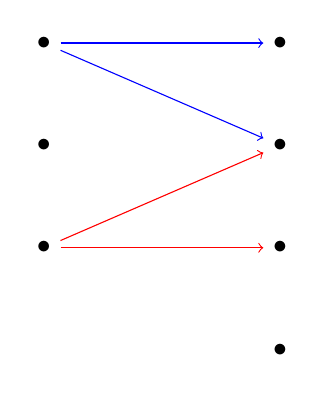
\begin{tikzpicture}[node distance = 1.3cm]
        % Nodes

        \node (X-1) {$\Large{\bullet}$};

        \node (X-2) [below of = X-1] {$\Large{\bullet}$};

        \node (X-3) [below of = X-2] {$\Large{\bullet}$};

        \node (Y-1) [right of = X-1, node distance =
        3cm]{$\Large{\bullet}$};

        \node (Y-2) [below of = Y-1] {$\Large{\bullet}$};

        \node (Y-3) [below of = Y-2] {$\Large{\bullet}$};

        \node (Y-4) [below of = Y-3] {$\Large{\bullet}$};

        % Arrows

        \path [draw=blue,->] (X-1) -> (Y-1);

        \path [draw=blue,->] (X-1) -> (Y-2);


        \path [draw=red,->] (X-3) -> (Y-2);

        \path [draw=red,->] (X-3) -> (Y-3);

      \end{tikzpicture}

    \end{center}

    Subjects who apply a cumulative reading should judge this
    \emph{true}
  \end{itemize}
\item as far as I can see, this is the best we can do: we have control
  conditions (cases 1 and 4) that would detect cumulative
  readings; but when they do we simply cannot use pictures like these
  to test cases 3 and 4 (if we wanted that, we'd need different visual
  material, unfortunately)
\item or am I wrong?
\item finally, if cumulative readings are possible for ``all of the
  $X$'s'' in (\ref{bsp:All_Some-Global}), so should they be in
  (\ref{bsp:Exactly_1_All-Global}), shouldn't they?
\item but here, too, we would see this in subjects responding
  \emph{true} in case 3 (as above) for this case\draftnote{careful: I
    mean the \emph{first} false-false picture; the previous text
    contained two times ``case 3'', a typo!}
\end{itemize}


\end{document}
